\pdfminorversion=4
\documentclass[]{article}

%%%%%%%%%%%%%%%%%%%
% Packages/Macros %
%%%%%%%%%%%%%%%%%%%
\usepackage{amssymb,latexsym,amsmath}     % Standard packages
\usepackage[norsk,portuges,latin,english,spanish,italian]{babel}
\usepackage[utf8]{inputenc}
\usepackage[T3,T1]{fontenc}
\usepackage[pdftex]{graphicx}
\usepackage{caption}
\usepackage{hyperref}


%%%%%%%%%%%
% Margini %
%%%%%%%%%%%
\addtolength{\textwidth}{1.0in}
\addtolength{\textheight}{1.00in}
\addtolength{\evensidemargin}{-0.75in}
\addtolength{\oddsidemargin}{-0.75in}
\addtolength{\topmargin}{-.50in}


%%%%%%%%%%%%%%%%%%%%%%%%%%%%%%
% Theorem/Proof Environments %
%%%%%%%%%%%%%%%%%%%%%%%%%%%%%%
\newtheorem{theorem}{Theorem}
\newenvironment{proof}{\noindent{\bf Proof:}}{$\hfill \Box$ \vspace{10pt}}  


%%%%%%%%%%%%
% Document %
%%%%%%%%%%%%
\begin{document}

\title{Low cost EC and pH meter for cavers}
\author{Luca Tringali}
\maketitle

\begin{abstract}
We started designing.
\end{abstract}

\section{Overview}

\section{Assembly guide}
\subsection{Parts}
Building one of these meters requires about 100 euros.

\begin{center}
\begin{tabular}{l||c|r}
Item & Price (avg.) & Notes \\ \hline
DFRobot EC module with probe & 31 & Version 1 \\
DFRobot pH module with probe & 25 & Version 1 \\
DS18B20 & 1.3 &  \\
Arduino MEGA R3 & 8 & \\
LCD 1602 I2C & 2.7 & \\
Keypad 4*5 & 2 & \\
Data Logger Shield & 2.5 & SD + RTC \\
10 KOhm resistor & 1 & 1 euro per 10 resistors \\
Dupont cables & 4 & mixed, m-m,f-m,f-f \\
Total & 77.5 & 
\end{tabular}
\end{center}


\subsubsection{Probes}
\begin{enumerate}
\item {Conductivity probe: DFRobot Gravity Electric Conductivity Kit K=1 \\(https://it.farnell.com/dfrobot/dfr0300/analog-electrical-conductivity/dp/2946108) (Versione precedente: Euro 34)  Euro 74 \\ Nota: il circuito è in grado di funzionare con qualsiasi cella di conducibilità dotata di attacco BNC. Non è necessario modificare il circuito. \\ \href{https://www.dfrobot.com/product-1797.html\#comment-4508952573}{Fonte} \\ Le celle più economiche sono prodotte da \href{http://web.archive.org/web/20200406124240im_/http://www.sinotester.com/Uploads/image/20180115/20180115084843_34419.jpg}{DJS}.
\\ Va però considerato che queste celle sono progettate per un utilizzo di laboratorio, è sconsigliabile tenerle immerse più di 3 ore in acqua altrimenti perdono affidabilità nel corso del tempo. Per monitoraggi in continuo che devono durare mesi, conviene puntare su celle per utilizzo industriale.}
\item {pH probe}
\item {Thermometer: DS18B20 Euro 1,3}
\end{enumerate}

\subsubsection{Electronics}
\begin{enumerate}
\item {Resistenza 10KOhm (Euro 1 pacco da 10 pezzi)}
\item {Cavi Dupont}
\item {Arduino MEGA R3 Euro 8}
\item {LCD 1602 I2C https://it.aliexpress.com/item/32685612494.html \\ https://win.adrirobot.it/rtc\_module/immagini/test\_rtc-DS1302\_bb.jpg}
\item {Keypad 4*5 https://it.aliexpress.com/item/4000145872100.html Euro 2}
\item {Data Logger Shield \\ Il datalogging shield richiede una pila CR1220 a 3V. Non è chiaro quanto duri, ma sicuramente alcuni anni.\\
Da notare che l'orologio viene reimpostato automaticamente aggiornando il firmware.}
\end{enumerate}

\subsubsection{Case}
\begin{enumerate}
\item {Scatola derivazione IP55 125x125x75 (https://it.aliexpress.com/item/32985090338.html, 8 euro) oppure 155x115x60}
\item {pH probe}
\item {Thermometer}
\end{enumerate}

\subsection{Connections}

You should use only dupont cables to connect Arduino pins. No soldering is required. Which is good if you need to quickly replace some parts due to failure, even while being outdoor.

{\centering  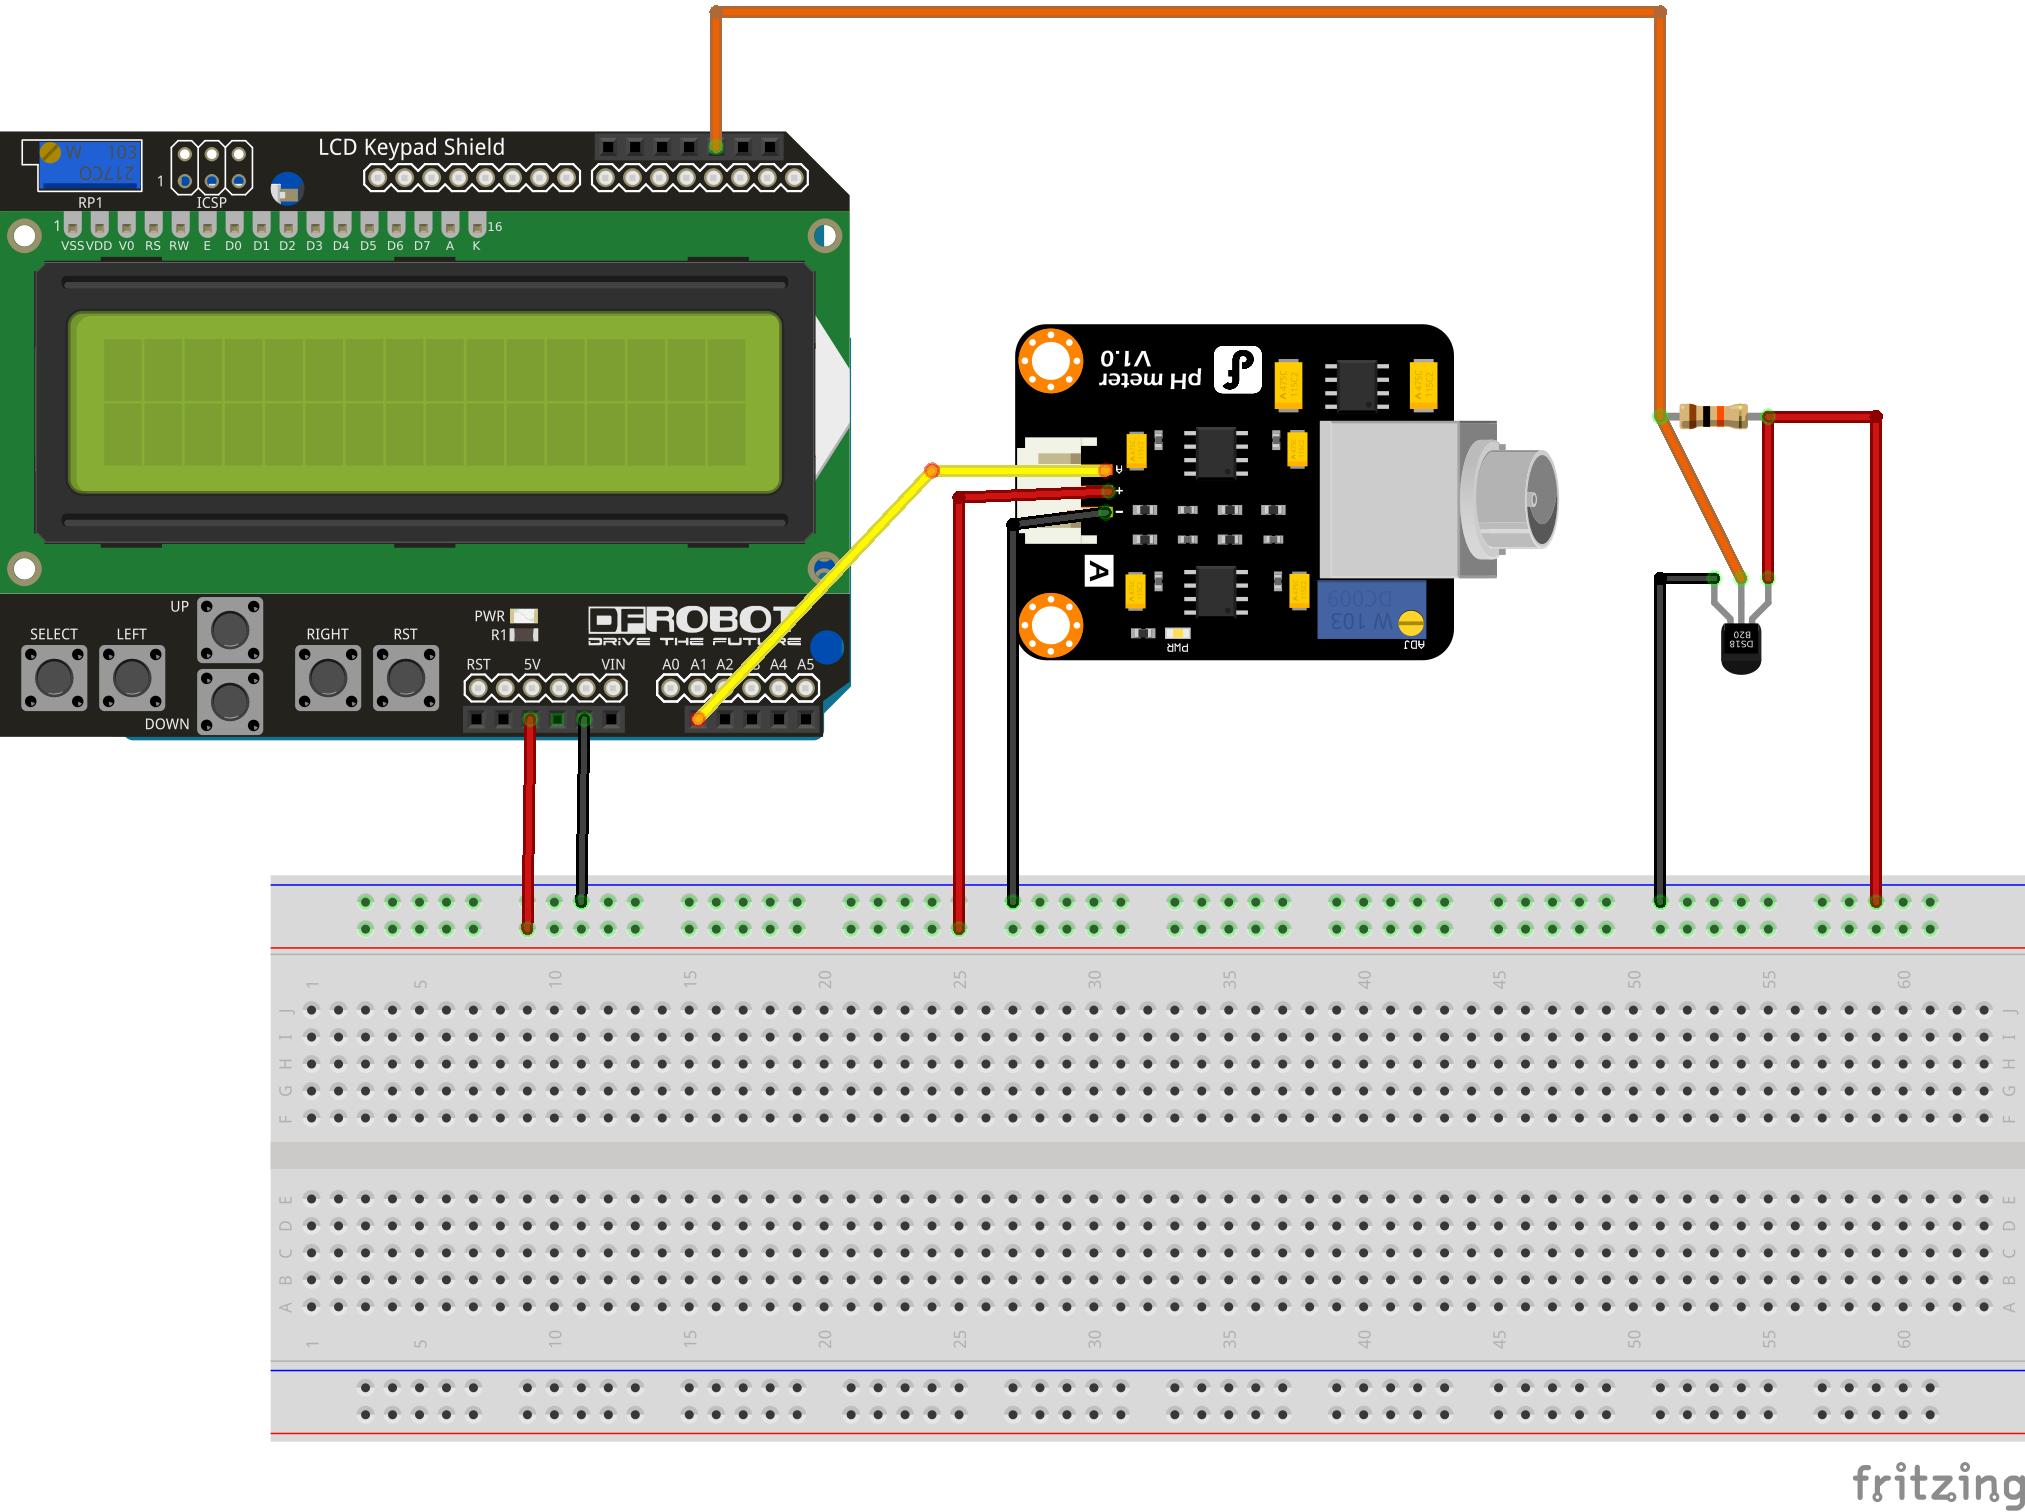
\includegraphics[width=0.9\textwidth]{foto_conduttimetro/conduttimetro_da_campo_bb.png} \par}
\captionof{figure}{Full schematic}

Qui scriviamo altre cose.

{\centering  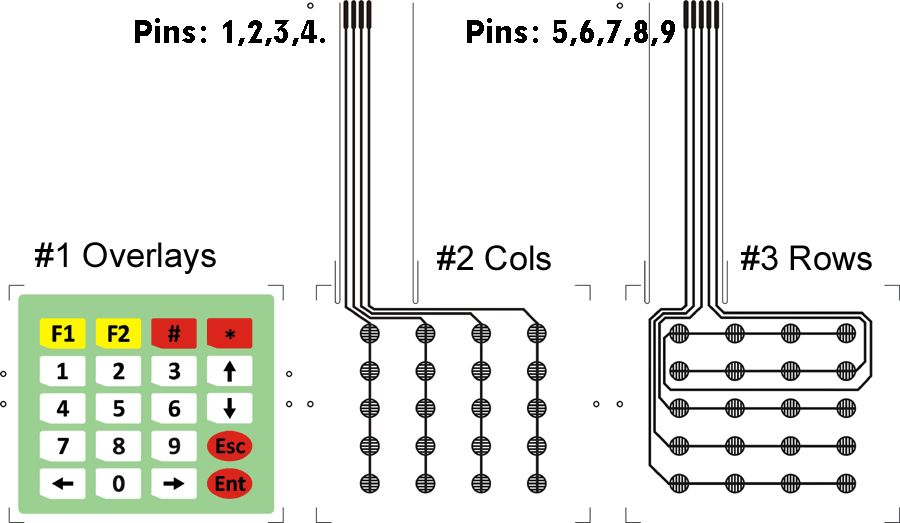
\includegraphics[width=0.9\textwidth]{foto_conduttimetro/keypad.jpg} \par}
\captionof{figure}{Punti di interesse per le acque carsiche}

Qui scriviamo altre cose.

\section{Programming}
Per poter compilare il codice è necessario avere installate queste librerie nel proprio Arduino IDE:
\begin{enumerate}
\item {EEPROM by Arduino}
\item {Wire by Arduino}
\item {SD\_MEGA by Arduino, Adafruit, Tringali}
\item {SPI by Arduino}
\item {DFRobot\_EC-master on https://github.com/DFRobot/DFRobot\_EC}
\item {DFRobot\_PH-master on https://github.com/DFRobot/DFRobot\_PH}
\item {DallasTemperature by Miles Burton et al}
\item {OneWire by Jim Studt et al}
\item {LiquidCrystal by Arduino, Adafruit}
\item {RTClib by Adafruit}
\item {Keypad library by Mark Stanley and Alexander Brevig}
\end{enumerate}

\section{Manual}
Attenzione: la lettura dei dati e il logging sono attivi solo mentre è visualizzata la schermata principale. Mentre si visualizza il menù, il datalogging è sospeso. \\
Per accedere al menù basta tenere premuto per 1 secondo il pulsante **Select**. Per scorrere le varie opzioni del menù si premono i tasti **Su** e **Giù**.
Esistono le seguenti opzioni:\\


\begin{enumerate}
\item { **Scrivi su SD**: mostra lo stato del datalogging, cioè la memorizzazione dei dati su scheda SD. Se appare un asterisco, il data logging è abilitato, altrimenti no. Per modificare l'impostazione (da disabilitato a abilitato e viceversa) basta premere il tasto **Select**.}
\item { **Media su numero s**: mostra il numero di secondi entro i quali viene eseguita la media. Per ridurre l'effetto della variabilità casuale, soprattutto in acque con flusso rapido, il processore esegue una media sui dati degli ultimi 10 secondi. Per cambiare il numero di secondi considerati basta premere le frecce **Destra** e **Sinistra**.}
\item { **HH:MM:SS DDMMYY**: mostra ora e data con due cifre per l'ora, due per i minuti, e due per i secondi, poi due per il giorno, due per il mese, e due per l'anno. Premendo il pulsante Select si può reimpostare data e ora, ma la funzione non è ancora implementata al momento.}
\item { **Calibrazione**: premendo **Select** il dispositivo entra in modalità seriale (USB) e attende il comando per la calibrazione. È necessario che il dispositivo sia connesso a un computer tramite porta USB.}
\item { **Reset memoria**: premendo **Select** si cancella la memoria EEPROM, eliminando i parametri di calibrazione del conduttimetro.}
\item { **Esci**: premendo **Select** si esce dal menù e si ritorna alla schermata principale.}
\end{enumerate}


\end{document}

%%%%%%%%%%%%%%%%%%%%%%%
%  TEMPLATES
%%%%%%%%%%%%%%%%%%%%%%%



\section{Lists}
%%%%%%%%%%%%%%%
\begin{enumerate}
\item {\bf First Point (Bold Face)}
\item {\em Second Point (Italic)}
\item {\Large Third Point (Large Font)}
    \begin{enumerate}
        \item {\small First Subpoint (Small Font)} 
        \item {\tiny Second Subpoint (Tiny Font)} 
        \item {\Huge Third Subpoint (Huge Font)} 
    \end{enumerate}
\item[$\bullet$] {\sf Bullet Point (Sans Serif)}
\item[$\circ$] {\sc Circle Point (Small Caps)} 
\end{enumerate}


\section{Equations}
%%%%%%%%%%%%%%%%%%%

\subsection{Binomial Theorem}
\begin{theorem}[Binomial Theorem]
For any nonnegative integer $n$, we have
$$(1+x)^n = \sum_{i=0}^n {n \choose i} x^i$$
\end{theorem}

\subsection{Taylor Series}
The Taylor series expansion for the function $e^x$ is given by
\begin{equation}
e^x = 1 + x + \frac{x^2}{2} + \frac{x^3}{6} + \cdots = \sum_{n\geq 0} \frac{x^n}{n!}
\end{equation}



\section{Tables}
%%%%%%%%%%%%%%%%
\begin{center}
\begin{tabular}{l||c|r}
left justified & center & right justified \\ \hline
1 & 3.14159 & 5 \\
2.4678 & 3 &  1234 \\ \hline \hline
3.4678 & 6.14159 & 1239
\end{tabular}
\end{center}


\section{A Picture}
%%%%%%%%%%%%%%%%%%%
\begin{center}
\begin{picture}(100,100)(0,0)
\setlength{\unitlength}{1pt}
\put(20,70){\circle{30}}  \put(20,70){\circle*{10}}   % left eye
\put(80,70){\circle{30}}  \put(80,70){\circle*{10}}   % right eye
\put(40,40){\line(1,2){10}} \put(60,40){\line(-1,2){10}} \put(40,40){\line(1,0){20}} % nose
\put(50,20){\oval(80,10)[b]} % mouth
\multiput(0,90)(4,0){10}{\line(1,3){4}}  % left eyebrow
\multiput(100,90)(-4,0){10}{\line(-1,3){4}}  % right eyebrow
\end{picture}
\end{center}


\section{A image from file}
%%%%%%%%%%%%%%%%%%%
{\centering  \includegraphics[width=0.9\textwidth]{028-capture.jpg} \par}
\captionof{figure}{Una immagine dei pipistrelli in Grotta Regina}


